% !TeX root = ../../main.tex
\section{Crystalliser design}

\subsection{(p-Nitrotoluene + m-nitrotoluene) phase behaviour}

The (p-NT + m-NT) system exhibits a eutectic-forming solid-liquid phase behaviour. In such system, depending on the composition, one of the two components is able to crystallise out from the homogeneous liquid as pure solid when the mixture is cooled below thermodynamic equilibrium. \cite{seader_separation_2011} Figure \ref{fig:eutectic schematic}a is a schematic of this process. Here, starting from point 1 on the solid-liquid phase boundary, which is on the right-hand-side of the eutectic point, the temperature is at $T_1$ with the fraction of component A at $x_1$. When the mixture is cooled down to $T_2$, at equilibrium, the liquid phase composition will become $x_2$. Since $x_2$ is lower than $x_1$, this means pure solid A would crystallise out from the liquid. The amount of solid A would be given by
\begin{equation}\label{eq:amount solid A equilibrium}
    \dot{M}_{solid} = \frac{\dot{M}_{total} (x_1 - x_2)}{1 - x_2}
\end{equation}
where $\dot{M}_{solid}$ is the equilibrium mass flow rate of crystallised solid A and $\dot{M}_{total}$ is the total mass flow rate of A and B. 

\begin{figure}[h]
    \centering
    \includesvg[scale=0.45,inkscapelatex=false]{figures/Eutectic_schematic.svg}
    \caption{(a) Schematic diagram for a typical eutectic-forming solid-liquid phase behaviour. (b) Solid-liquid phase diagram for the (p-NT + m-NT) system.}
    \label{fig:eutectic schematic}
\end{figure}

Figure \ref{fig:eutectic schematic}b is a plot of the solid-liquid phase diagram for the (p-NT + m-NT) system, where the component fraction on the horizontal axis has been defined for p-NT. Experimental data were obtained from \cite{noauthor_detherm_2021} and are marked on this Figure as green circles. For the purpose of design, a model that is able to continuously predict the phase behaviour is needed. Initially, a van't Hoff-type relation from Moyers and Rousseau was used to give continuous predictions of the solid-liquid phase boundary on the right-hand-side of the eutectic point, \cite{moyers_crystallization_1987}
\begin{equation}
    ln(x) = \frac{H_{fusion}}{R T}(\frac{T}{T_{melt}} - 1)
\end{equation}
where $x$ is the fraction of p-NT, $H_f$ is the heat of fusion when p-NT melts, $T$ is the equilibrium temperature, and $T_{melt}$ is the melting point of pure p-NT. However, as can be seen on Figure \ref{fig:eutectic schematic}b, predictions of Moyers and Rousseau's van't Hoff relation, shown as the red curve, are quite off from experimental data. In particular, this relation over-predicts the melting temperature at compositions approaching the eutectic point. A better description is thus necessary, and a van't Hoff-type power-law fit has been devised instead in the form of 
\begin{equation}
     ln(x) = \frac{T - 323.87}{50.259}
\end{equation}

It has been found that this fitted correlation would give an $R^2$ of 0.9901 against experimental data; indeed, as can be seen on Figure \ref{fig:eutectic schematic}b, predictions from this correlation, shown as the blue curve, do fit well with the experimental results, hence it has been applied for the design.

In reality, the system needs time to reach thermodynamic equilibrium from where it starts off, which is why a physical crystalliser is needed. Kinetics of crystallisation in a MSMPR crystalliser will be explained in the following sections.

\subsection{Kinetics of MSMPR crystallisation}
The kinetics of crystallisation is governed by two processes: nucleation and growth. Nucleation is the genesis of embryo-sized crystals known as nuclei due to supersaturation. \cite{richardson_chemical_nodate} It is further classified into primary and secondary nucleation. Growth is the process of existing crystals growing in size, where the material diffuses and deposits on the surface of the crystal and make it grow in volume. During crystallisation, these two processes happen simultaneously, both contributing to the final crystal size distribution (CSD). \cite{richardson_chemical_nodate} They are not, however, independent of each other: nucleation provides nuclei whereon crystal growth can occur. For unseeded crystallisation, nucleation is the first step of crystallisation, and growth happens after nuclei are formed. \cite{mullin}

\subsubsection{Supersaturation}

Before nucleation and crystal growth are elaborated in further details, the concept of supersaturation must be established. Supersaturation is the driving force for both nucleation and growth, and it is a measure of how much the system is off from equilibrium. Several measures exist that are able to describe the degree of supersaturation. The commonest definition is expressed as a difference in concentration from equilibrium,

\begin{equation}
    \Delta C = C - C_{eq}
\end{equation}

where $C$ is the actual concentration of crystallising component in the liquid at any point in time, and $C_{eq}$ is the equilibrium concentration corresponding to the operated temperature of the system. Alternatively, it can be defined as a ratio, where

\begin{equation} \label{eq: supersaturation ratio}
    S = \frac{C}{C_{eq}}
\end{equation}

and $S$ is known as the supersaturation ratio. A third way of defining supersaturation is on a temperature basis, where the quantity known as degree of super-cooling can be defined such that

\begin{equation}
     \Delta T = T - T_{eq}
\end{equation}

\noindent whence $T$ is the equilibrium temperature corresponding to concentration $c$ in the liquid, and $T_{eq}$ is the operated temperature to which the system has been super-cooled. Figure \ref{fig:supersaturation} is a schematic which explains these relations.

\begin{wrapfigure}{r}{0.5\linewidth}
\centering
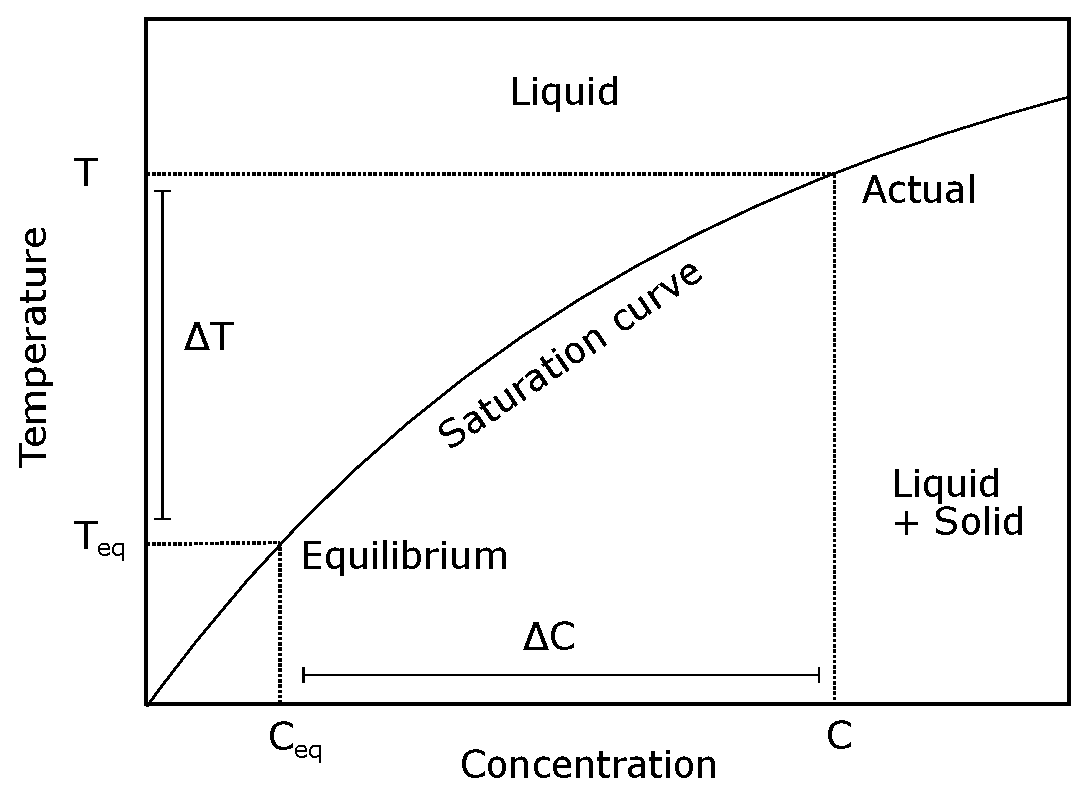
\includegraphics[scale=.3]{chapters/3-separation/figures/Supersaturation.eps}
\caption{A schematic diagram showing the definitions of supersaturation.}
\label{fig:supersaturation}
\end{wrapfigure}


\subsubsection{Primary nucleation}

Primary nucleation involves nucleation occurring in absence of crystals. \cite{seader_separation_2011} It can be further classified into homogeneous nucleation and heterogeneous nucleation. The former is where nuclei are formed from supersaturation only, and the latter results from the presence of insoluble materials. \cite{richardson_chemical_nodate} The rate at which homogeneous rate of nucleation happens is typically given by an Arrhenius-type expression, \cite{richardson_chemical_nodate}

\begin{equation}
     J = F~exp(-\frac{16 \pi \sigma^3 \nu^2}{3 k^3 T^3 (ln~S)^2})
\end{equation}

where $J$ is the rate of primary nucleation in  $F$ is a pre-exponential factor, $\sigma$ is the interfacial tension between the crystal and the surrounding supersaturated liquid, $T$ is the temperature, $\nu$ is the molar volume, $k$ is the Boltzmann constant, and $S$ is the supersaturation ratio defined in Equation \ref{eq: supersaturation ratio}. The pre-exponential factor, $F$, is a function of supersaturation. It is estimated to be in the order of magnitude of 10$^{30}$ cm$^{-3}$s$^{-1}$ by Randolph and Larson. \cite{randolph_theory_1971} Compared to secondary nucleation, primary nucleation is numerically negligible for industrial applications and hence has been omitted from design calculations. 

\subsubsection{Secondary nucleation}

Secondary nucleation takes place when crystals of the species are already present. \cite{richardson_chemical_nodate} When no seeding is introduced, contact secondary nucleation between the existing crystals themselves or between the crystals and the walls and stirrer are the most significant. 

\subsubsection{Crystal growth}

Alongside the mass balance, the phenomenon of crystal growth is governed by the crystal population balance. The population balance, together with the mass balance, accounts for the crystal size distribution (CSD) where important information about the growth kinetics is contained. It has been a central focus in the works of Randoph and Larson. \cite{randolph_theory_1971}

First, for many commercial crystallisation processes, McCabe's $\Delta L$  law is a general constraint,
\begin{equation} \label{eq: McCabe deltaL}
    \Delta L = G \Delta t
\end{equation}
where $L$ is the characteristic size of crystal, $t$ is time, and $G$ is the growth rate whose dimensions are length per unit time. The main underlying assumption is that the crystal growth rate is independent of crystal size. 

Then, the crystal population density, $n$, defined as the number of crystals per unit size per unit volume, is expressed as 
\begin{equation} \label{eq:crystal population density definition}
    .
\end{equation}






\subsection{Heat transfer}

The crystallisation cooling can be implemented many different ways and must be chosen based on the conditions of the crystalliser. Table \ref{tab:heatransfermethodstype} outline the properties of each heat transfer method. A half pipe coil jacketed vessel configuration was implemented as this method exhibits excellent heat transfer capability, especially when the service side fluid is a liquid, and despite usually costing 30-35\% more than conventional jackets, this is outweighed by the decreased operating cost and improved heat transfer. An impeller would also ensure good mixing, assumed to be perfect, to have uniform temperature within the crystalliser. 

\begin{table}
\caption{Comparison of heat transfer methods \cite{myerson_handbook_2019} }
\label{tab:heatransfermethodstype}
\begin{tabularx}{\linewidth}{lXX}
\toprule
Type & Advantages                 & Disadvantages                               \\ \midrule
Conventional Jacket & \begin{itemize}[label=+,leftmargin=1em]
  \item Achieves maximum coverage of shell and bottom of the vessel
  \item Accommodate heavier corrosion allowances
\end{itemize} & \begin{itemize}[label=-,leftmargin=1em]
  \item Poor heat transfer due to low flow media velocity
  \item External pressure from jacket can require higher vessel wall thickness 
\end{itemize} \\\midrule 
Dimple Jacket & \begin{itemize}[label=+,leftmargin=1em]
  \item Dimples introduce turbulence in the cooling media flow
  \item Does not require thicker vessel wall from external jacket pressure
\end{itemize} & \begin{itemize}[label=-,leftmargin=1em]
  \item Thinner wall does not allow for heavier corrosion allowances
  \item Difficult to repair
  \item Fabrication is labor intensive
\end{itemize} \\\midrule
Half pipe coil  &  \begin{itemize}[label=+,leftmargin=1em]
  \item Excellent heat transfer
  \item Withstands higher jacket pressures
\end{itemize} & \begin{itemize}[label=-,leftmargin=1em]
  \item Problematic when trying to route around ports and supports 
  \item More expensive than conventional jackets

\end{itemize}
\\\bottomrule
\end{tabularx}
\end{table}

The following equation were solved simulantaneously in MATLAB 


To calculate the required length of half coil piping, the total heat transfer needs to be quantified first. Assuming complete heat transfer to the pipe and coolant, the total heat flow from the process side to the coolant media is calculated from:
\begin{equation} \label{eq:energy balance}
    Q =  \Dot{m}_{f}C_{pi}(T_{in}-T_{out})+ \Delta H_{C}\Dot{m}_{c}
\end{equation}
where Q is the total heat flow, $\Dot{m}_f$ is the feed mass flow rate, $C_{pi}$ is the specific heat capacity of the mixture, $\Delta H_{C}$ is the enthalpy of crystallisation, $\Dot{m}_{c}$ is the product crystal flow rate and the $T_{in}$ and $T_{out}$ are the inlet and outlet temperatures of the MSMPR respectively.


The overall heat transfer coefficient consists of 4 resistance terms; $R_1$, $R_w$, $R_2$ and $R_f$.
\begin{equation} \label{eq:resistht}
    R_O = R_1 + R_w + R_2 + R_f
\end{equation}
where $R_1$ is the process side convective heat transfer term, $R_w$ is the conductive heat transfer, $R_2$ is the service side convective heat transfer, $R_f$ the additional resistance due to fouling. In these calculations, any resistance due to fouling is not taken into accountant, but the effects are investigated in depth in later sections. %label section with fouling sensitiivty%.

Accounting for all these resistances in series, the overall heat transfer coefficient is obtained  
\begin{equation} \label{eq:energy balance}
    U = \left(\frac{1}{h_1} + \frac{l}{k}   + \frac{1}{h_2 } \right)^{-1}
\end{equation}
where l is the thickness of the half coil pipe, k is the thermal conductivity of pipe material (steel)

To determine the heat transfer coefficients on both the process side, Equation \ref{eq:processsideht}, and service side, Equation \ref{eq:servicesideht}, Nusselt number for a jacketed vessel with impeller agitator was used.
\begin{align} 
    \mathrm{Nu} &= A\mathrm{Re}^{\frac{2}{3}}\mathrm{Pr}^{\frac{1}{3}}\left( \frac{\eta}{\eta_w} \right)^{0.14} \label{eq:processsideht} \\
    \mathrm{Nu} &= 0.023\mathrm{Re}^{0.8}\mathrm{Pr}^{\frac{1}{3}} \left( \frac{\eta}{\eta_w} \right)^{0.14} \label{eq:servicesideht}
\end{align}

where A is the impeller constant, 0.611 in this case. From these equations, the respective heat transfer coefficients are used in the equation for the overall coefficient, U.



The equation for the heat transfer area was formulated using the length of the helix and the circumference of the service side half pipe, yielding:

\begin{equation} \label{eq:coolantpipesa}
    A_s = \frac{\pi D_p L}{2}
    \end{equation}
    
\begin{equation}\label{eq:helixlength}
    L = N \sqrt{C^2 + P^2}
\end{equation}

where L is the total length of the half pipe, N is the number of revolutions in the helix, C is the circumference of the coiling and P is the "pitch" or height of a single coil. The length and circumference of the pipe is then used



